\subsubsection{Rancangan Detail Subsistem Penyimpanan}
\label{subsubsection:detail-subsistem-penyimpanan}

Subsistem penyimpanan adalah subsistem yang bertanggung jawab untuk fungsionalitas \textit{key-value store} dalam sebuah \textit{Node}. Subsistem ini akan terdiri atas komponen \textit{in-memory store}, \textit{persistent store}, \textit{transaction log}. Subsistem ini juga mengkonfigurasi \textit{Node} untuk menggunakan replikasi atau \textit{erasure coding}. Ilustrasi struktur subsistem penyimpanan dapat dilihat pada gambar \ref{fig:storage-subsystem-structure}.

% _TODO: Change image
\begin{figure}[ht]
    \centering
    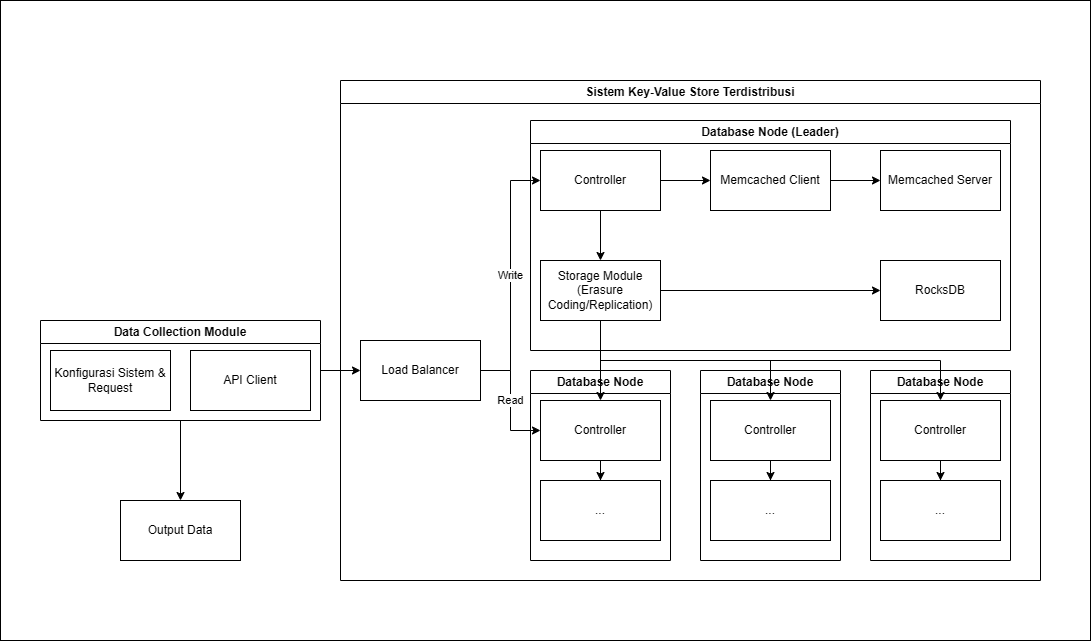
\includegraphics[width=0.95\textwidth]{resources/chapter-3/general-architecture.png}
    \caption{Struktur Subsistem Penyimpanan}
    \label{fig:storage-subsystem-structure}
\end{figure}
